%%%%%%%%%%%%%%%%%%%%%%%%%%%%%%%%%%%%%%%%%
% baposter Landscape Poster
% LaTeX Template
% Version 1.0 (11/06/13)
%
% baposter Class Created by:
% Brian Amberg (baposter@brian-amberg.de)
%
% This template has been downloaded from:
% http://www.LaTeXTemplates.com
%
% License:
% CC BY-NC-SA 3.0 (http://creativecommons.org/licenses/by-nc-sa/3.0/)
%
%%%%%%%%%%%%%%%%%%%%%%%%%%%%%%%%%%%%%%%%%

%----------------------------------------------------------------------------------------
%	PACKAGES AND OTHER DOCUMENT CONFIGURATIONS
%----------------------------------------------------------------------------------------

\documentclass[landscape,a0paper,fontscale=0.290]{baposter} % Adjust the font scale/size here

\usepackage{graphicx} % Required for including images
\graphicspath{{figures/}} % Directory in which figures are stored

\usepackage{amsmath} % For typesetting math
\usepackage{amssymb} % Adds new symbols to be used in math mode

\usepackage{booktabs} % Top and bottom rules for tables
\usepackage{enumitem} % Used to reduce itemize/enumerate spacing
\usepackage{palatino} % Use the Palatino font
\usepackage[font=small,labelfont=bf]{caption} % Required for specifying captions to tables and figures

\usepackage{multicol} % Required for multiple columns
\setlength{\columnsep}{1.5em} % Slightly increase the space between columns
\setlength{\columnseprule}{0mm} % No horizontal rule between columns

\usepackage{tikz} % Required for flow chart
\usetikzlibrary{shapes,arrows} % Tikz libraries required for the flow chart in the template

\newcommand{\compresslist}{ % Define a command to reduce spacing within itemize/enumerate environments, this is used right after \begin{itemize} or \begin{enumerate}
\setlength{\itemsep}{1pt}
\setlength{\parskip}{0pt}
\setlength{\parsep}{0pt}
}

\definecolor{lightblue}{rgb}{0.145,0.6666,1} % Defines the color used for content box headers

\begin{document}

\begin{poster}
{
headerborder=closed, % Adds a border around the header of content boxes
colspacing=1em, % Column spacing
bgColorOne=white, % Background color for the gradient on the left side of the poster
bgColorTwo=white, % Background color for the gradient on the right side of the poster
borderColor=lightblue, % Border color
headerColorOne=black, % Background color for the header in the content boxes (left side)
headerColorTwo=lightblue, % Background color for the header in the content boxes (right side)
headerFontColor=white, % Text color for the header text in the content boxes
boxColorOne=white, % Background color of the content boxes
textborder=roundedleft, % Format of the border around content boxes, can be: none, bars, coils, triangles, rectangle, rounded, roundedsmall, roundedright or faded
eyecatcher=true, % Set to false for ignoring the left logo in the title and move the title left
headerheight=0.15\textheight, % Height of the header
headershape=roundedright, % Specify the rounded corner in the content box headers, can be: rectangle, small-rounded, roundedright, roundedleft or rounded
headerfont=\Large\bf\textsc, % Large, bold and sans serif font in the headers of content boxes
%textfont={\setlength{\parindent}{1.5em}}, % Uncomment for paragraph indentation
linewidth=2pt % Width of the border lines around content boxes
}
%----------------------------------------------------------------------------------------
%	TITLE SECTION 
%----------------------------------------------------------------------------------------
%
{
\includegraphics[height=4em]{SB_Logo.png}} % First university/lab logo on the left
{\bf\textsc{Studying Deep Inelastic Scattering in e-p Collisions for a Future Electron-Ion Collider}\vspace{0.5em}} % Poster title
{\textsc{\ Daniel Bhatti, Sean Jeffas, \textbf{Thomas Krahulik}, \textbf{Joshua LaBounty}, \\ Rourke Sekelsky, Abhay Deshpande, Nils Feege \\ Stony Brook University Department of Physics and Astronomy}}% Author names and institution
{\hspace{10mm} \includegraphics[height=8em]{eiclogo.eps}} % Second university/lab logo on the right

%----------------------------------------------------------------------------------------
%	Electron Ion Collider
%----------------------------------------------------------------------------------------

\headerbox{Background}{name=EIC,column=0,row=0}{

A future Electron Ion Collider (EIC) would enable an investigation into the internal structure of protons and neutrons through the collision of electrons with protons or light ions. The process of probing the inside of a hadron by scattering an electron (or other lepton) off a quark inside that hadron is known as Deep Inelastic Scattering (DIS). An EIC detector is crucial to taking measurements of DIS events. 
%\begin{multicols}{2}
%\begin{center}
%\includegraphics[width=0.6\linewidth]{}
%\captionof{figure}{}
%\end{center}
%\begin{center}
%\includegraphics[width=0.6\linewidth]{Color_Glass.png}
%\captionof{figure}{LABEL}
%\end{center}
%\end{multicols}

%\vspace{0.3em} % When there are two boxes, some whitespace may need to be added if the one on the right has more content
}

%----------------------------------------------------------------------------------------
%	DIS Physics
%----------------------------------------------------------------------------------------

%\headerbox{Pythia Simulation}{name=method,column=0,below=objectives,bottomaligned=conclusion}{ % This block's bottom aligns with the bottom of the conclusion block
\headerbox{Theory}{name=method,column=0,below=EIC}{
\begin{center}
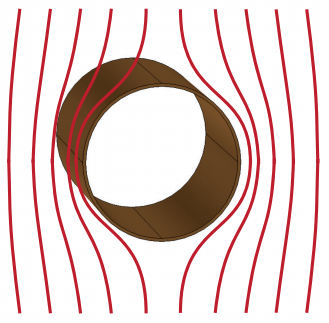
\includegraphics[width=0.45\linewidth]{ShieldConcept.png}
\captionof{figure}{Superconductor Shield Theory}
\end{center}

\begin{center}
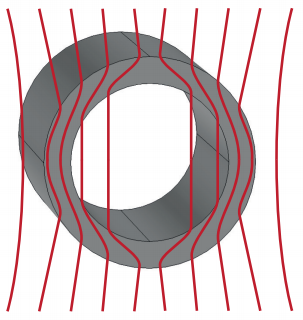
\includegraphics[width=0.45\linewidth]{Ferromagnet-Concept.png}
\captionof{figure}{Ferromagnet Theory}
\end{center}

\begin{center}
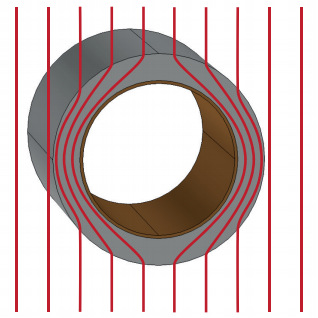
\includegraphics[width=0.45\linewidth]{CloakConcept.png}
\captionof{figure}{Magnetic Cloak Theory}
\end{center}


}

%----------------------------------------------------------------------------------------
%	Pythia Simulation
%----------------------------------------------------------------------------------------

\headerbox{Superconductor Shielding}{name=introduction,column=1,span=2,row=0}{
\begin{multicols}{3}
\begin{center}
\includegraphics[width=1.0\linewidth]{Pythia_peta_e_10M_250x010.png}
\captionof{figure}{Momentum Distribution of Electrons as a Function of Pseudorapidity $\eta$}
\end{center}
\begin{center}
\includegraphics[width=1.0\linewidth]{LepA.png}
\captionof{figure}{Distribution of $e^{-}$ as a Function of $x$ and $Q^2$ Compared to its Scattering Angle}
\end{center}
\begin{center}
\includegraphics[width=1.0\linewidth]{LOI_Rep_Q2x_K.png}
\captionof{figure}{Distribution of Kaons as a Function of $x$ and $Q^2$}
\end{center}
\end{multicols}

\normalsize An important step in the process of designing an EIC detector is the simulation of the electron-proton collisions that would occur within the collider. We use a simulation software known as Pythia 6, a Monte-Carlo event generator for high energy particle collisions. Simulated data can also be input into other types of software to perform an analysis of detector acceptance and performance.

}

%----------------------------------------------------------------------------------------
%	Radiative Corrections using RADGEN
%----------------------------------------------------------------------------------------

%\headerbox{Pythia Analysis}{name=results,column=2,span=2,row=0}{
\headerbox{Travel Opportunities}{name=results,column=3,row=0}{
In electron-proton collisions it is important to account for a photon that is radiated from the electron as it nears the proton. This emitted photon will slightly change the the kinematics of the electron and therefore the rest of the collision kinematics. Therefore we need to account for the photon's energy and angle in order to correct the kinematics for the electron, and the rest of the collision. The equations to calculate these corrections are shown below.

\begin{center}
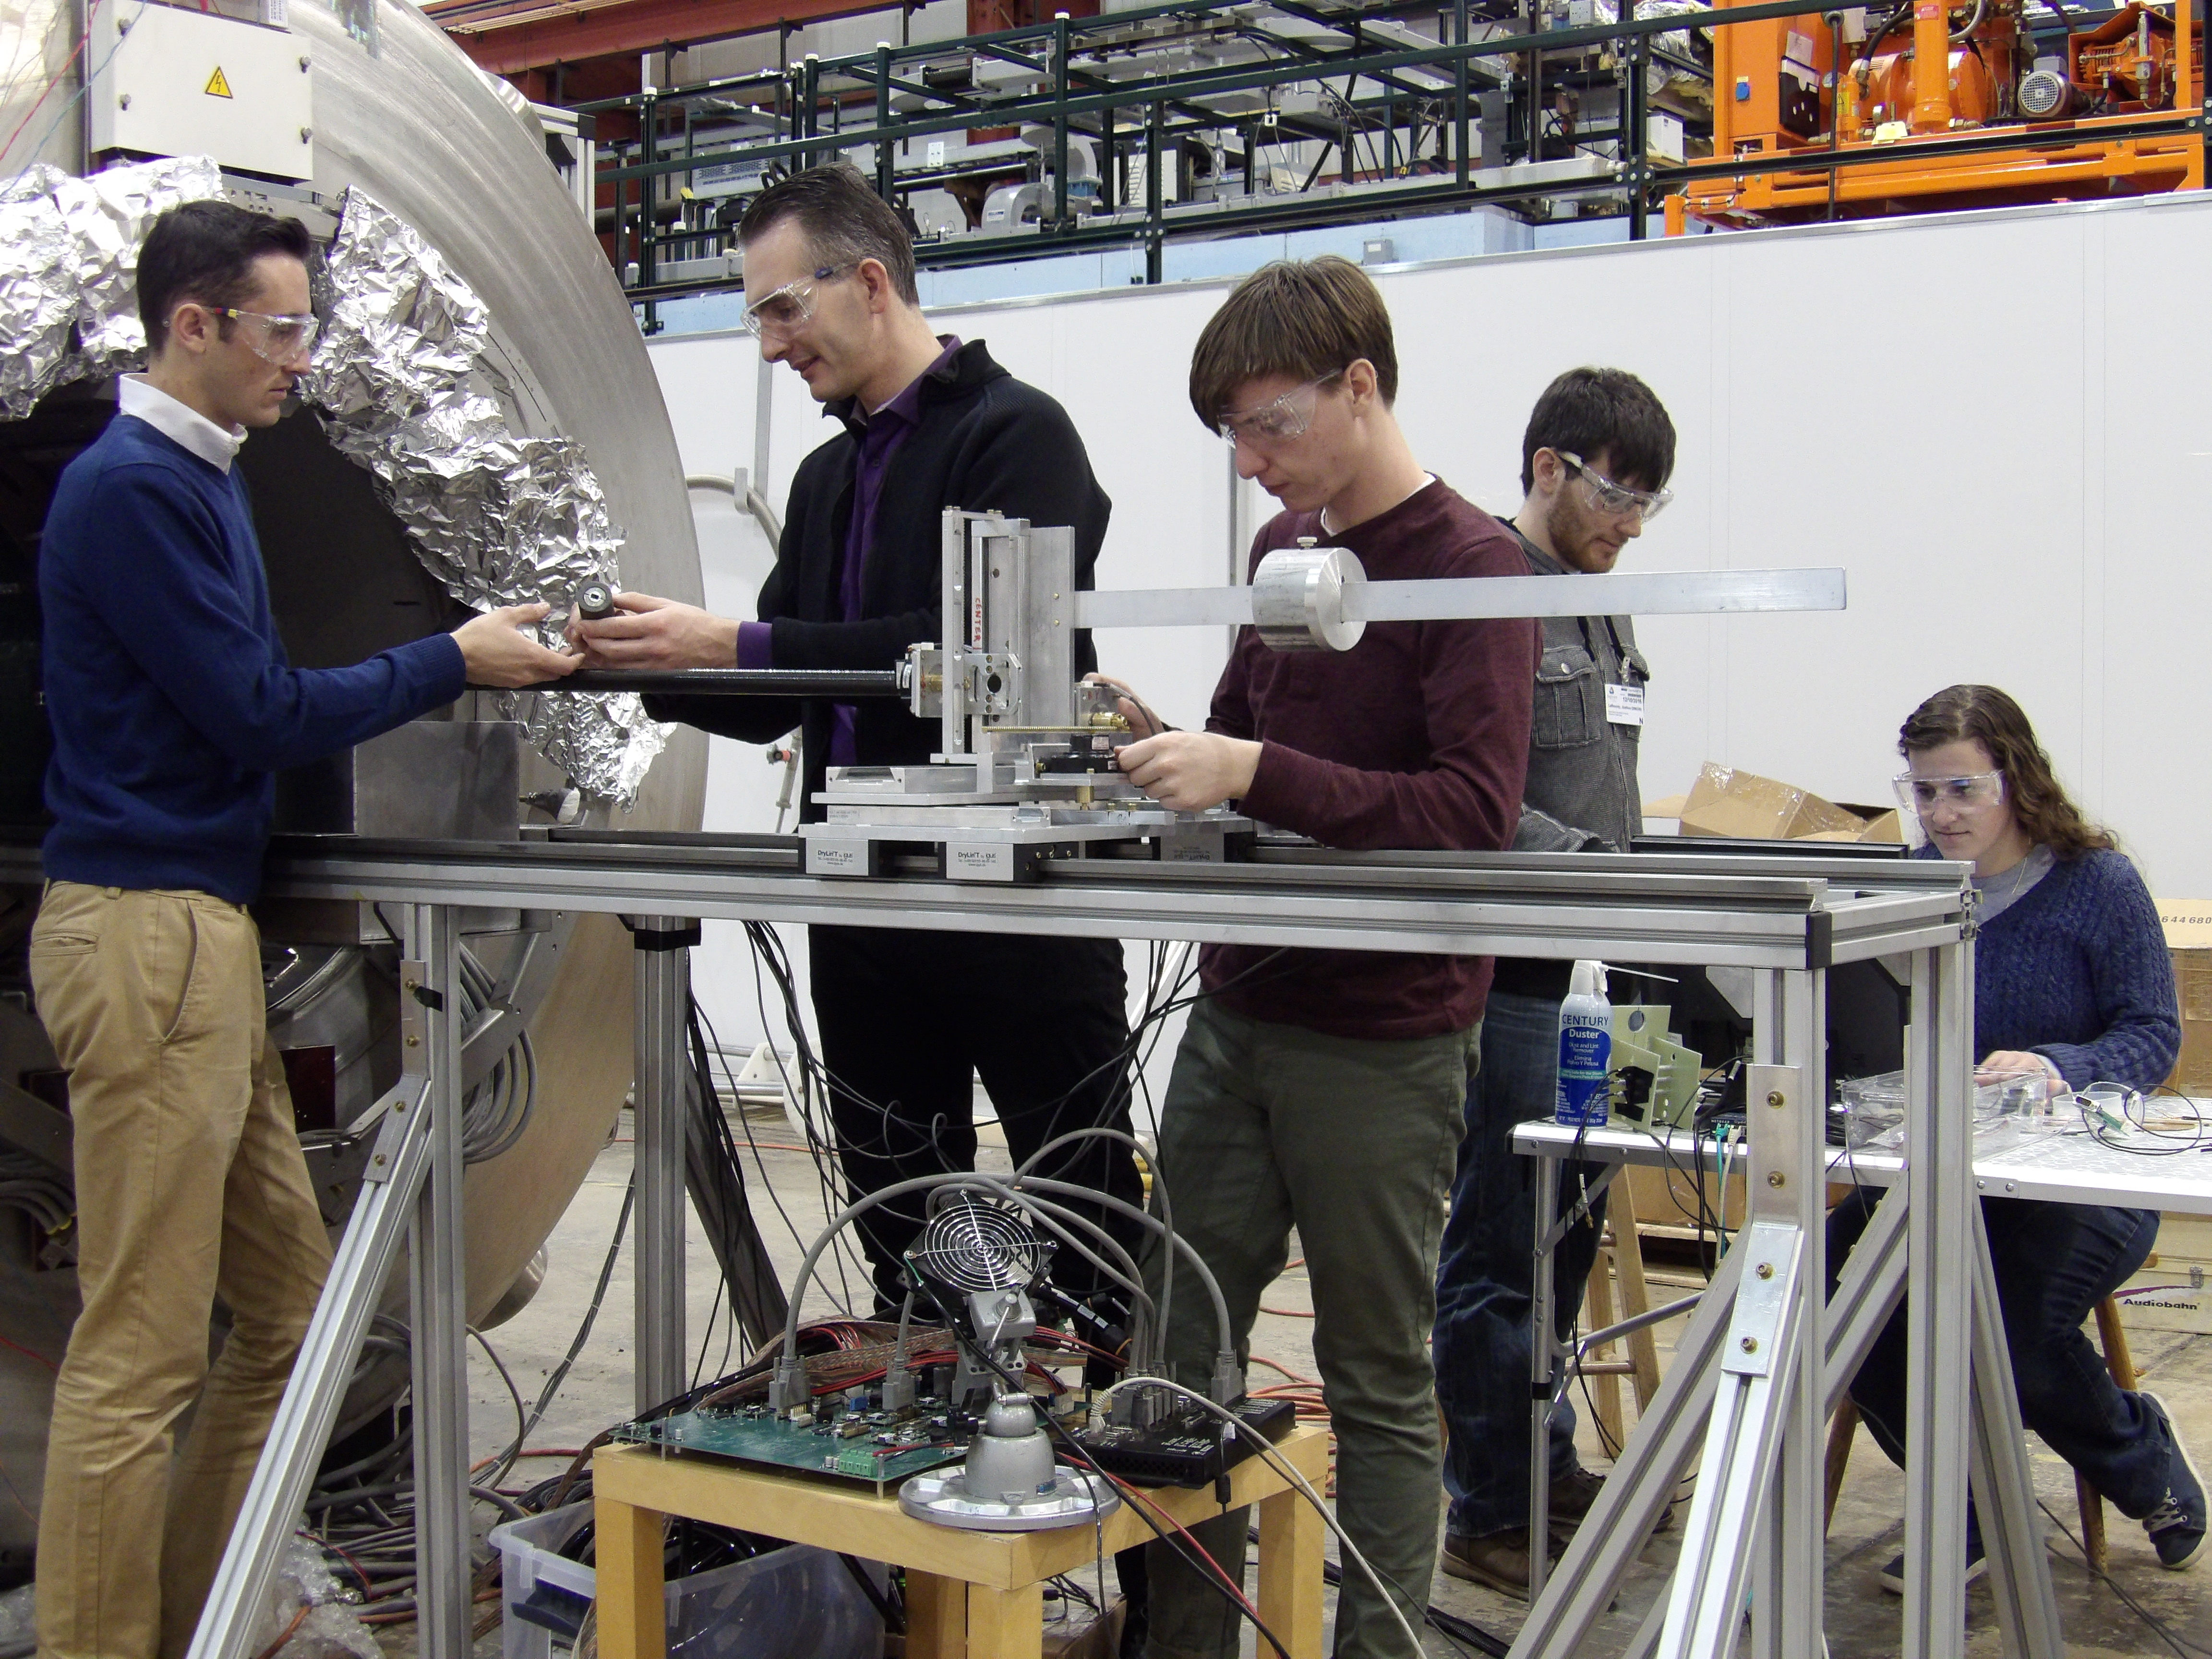
\includegraphics[width=0.7\linewidth]{ANL-Pic.JPG}
\captionof{figure}{Measuring magnetic field cloaking at Argonne National Lab}
\end{center}
\vspace{-2mm}
\large \begin{equation}
Q_{true}^{2} = Q^2 + 2E_{\gamma} (\nu \sqrt{\nu^{2} + Q^2} cos(\theta_{\gamma}))
\end{equation}
\large \begin{equation}
x_{true} = \frac{Q_{true}^2}{2M \nu_{true}}
\end{equation}

\normalsize In order to account for these radiative corrections in simulations of electron-proton collisions, we use another event generator known as RADGEN which can calculate the true kinematics of the collisions.
}

%----------------------------------------------------------------------------------------
%	REFERENCES
%----------------------------------------------------------------------------------------

%\headerbox{References}{name=references,column=0,above=bottom}{

%\renewcommand{\section}[2]{\vskip 0.05em} % Get rid of the default "References" section title
%\nocite{*} % Insert publications even if they are not cited in the poster
%\small{ % Reduce the font size in this block
%\bibliographystyle{unsrt}
%\bibliography{sample} % Use sample.bib as the bibliography file
%}}

%----------------------------------------------------------------------------------------
%	References
%----------------------------------------------------------------------------------------

%\headerbox{Contact Information}{name=contact,column=3,aligned=references,above=bottom}{ % This block is as tall as the references block
\headerbox{References}{name=contact,column=3,above=bottom}{ % This block is as tall as the references block
\footnotesize \begin{enumerate}
\item Accardi, A., et al., \textit{Electron Ion Collider: The Next QCD Frontier} arXiv:1212.1701v3(2014)
\item Akushevich, I., H. Bottcher, D. Ryckbosch, \textit{RADGEN 1.0: Monte Carlo Generator for Radiated Events in DIS on Polarized and Unpolarized Targets} arXiv:hep-ph/9906408v1(1999)
\item PHENIX Collaboration, \textit{Concept for an Electron Ion Collider (EIC) detector built around the BaBar solenoid} arXiv:1402.1209v1(2014)
\item Wolf, G. \textit{HERA Physics} DESY 94-022 (1994).
\end{enumerate}
}

%----------------------------------------------------------------------------------------
%	Further Research
%----------------------------------------------------------------------------------------

%\headerbox{Geant4 Analysis}{name=conclusion,column=2,span=2,row=0,below=results,above=references}{
%\headerbox{Further Research}{name=conclusion,column=3,row=0,below=results}{

%\begin{multicols}{2}

%\end{multicols}
%}


%----------------------------------------------------------------------------------------
%	Geant4 Simulation
%----------------------------------------------------------------------------------------

\headerbox{Magnetic Field Cloaking}{name=results2,column=1,span=2,below=introduction,bottomaligned=contact}{ % This block's bottom aligns with the bottom of the conclusion block
\begin{multicols}{2}
\begin{center}
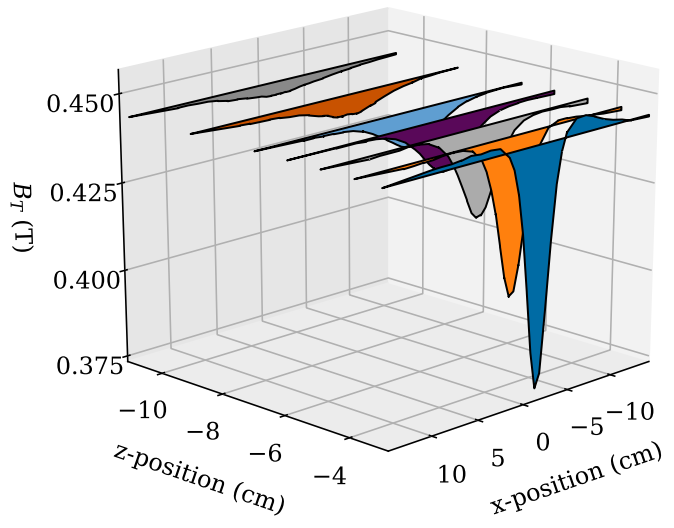
\includegraphics[width=1.0\linewidth]{NoCloak.png}
\captionof{figure}{MRI Field with Superconductor Shield}
\end{center}
\begin{center}
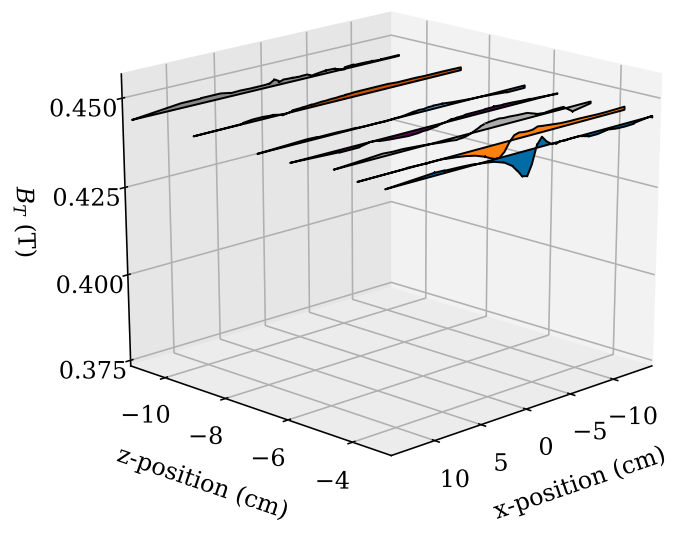
\includegraphics[width=0.95\linewidth]{WithCloak.png}
\captionof{figure}{MRI Field with Magnetic Field Cloak}
\end{center}
\end{multicols}


}

%----------------------------------------------------------------------------------------

\end{poster}

\end{document}